\chapter{Experimental Evaluation}
\label{chap:5}

\section{Introduction}
\label{sec:eval-intro}

With comparable I2C WASI interface implementations now available for both WAMR and Wasmtime runtimes, this chapter presents a comprehensive experimental evaluation comparing their \textbf{performance characteristics} and \textbf{resource utilization}. The primary focus centers on a detailed comparative analysis between these two WebAssembly runtime approaches, while leveraging the native implementation as a performance baseline and reference point.

The evaluation encompasses \textbf{timing analysis} across multiple execution phases and comprehensive \textbf{memory profiling} to track allocation patterns. This data is then used for statistical analysis to ensure reliable and reproducible results. By systematically measuring runtime setup overhead, execution latency, and memory consumption, this experimental evaluation provides quantitative insights into the practical trade-offs between different WebAssembly runtime architectures.

This analysis directly addresses the second research question of this thesis: \textbf{RQ2: What is the performance impact of different WebAssembly runtime approaches?} Through controlled experimentation and statistical validation, the evaluation establishes an empirical foundation for understanding when and why specific runtime choices are optimal for embedded I2C applications.

\section{Experimental Setup}
\label{sec:experimental-setup}
Having established the evaluation objectives and methodology in Section~\ref{sec:eval-intro}, this section details the required infrastructure. The experimental setup encompasses three critical components: the hardware configuration that enables I2C communication, the firmware implementations of the I2C peripheral, and the software framework that facilitates accurate performance measurement and statistical analysis.

\subsection{Hardware Configuration}
\label{subsec:hardware-config}

The experimental testbed consists of a Raspberry Pi acting as the I2C controller, connected to an Arduino Uno serving as the I2C peripheral.

\textbf{Controller Configuration:}
\begin{itemize}
    \item Board: \textit{Raspberry Pi 5}
    \item Architecture: \textit{ARM64} % TODO: reference pi datasheet
    \item Operating System: \textit{Raspberry Pi OS}
\end{itemize}

\textbf{Peripheral Configuration:}
\begin{itemize}
    \item Board: \textit{Arduino Uno R3 (ATmega328P)}
    \item Peripheral Address: \textit{0x09}
    \item Serial Interface: \textit{USB serial for correctness verification (disabled during performance tests)}
\end{itemize}

\begin{figure}[h]
	\centering
	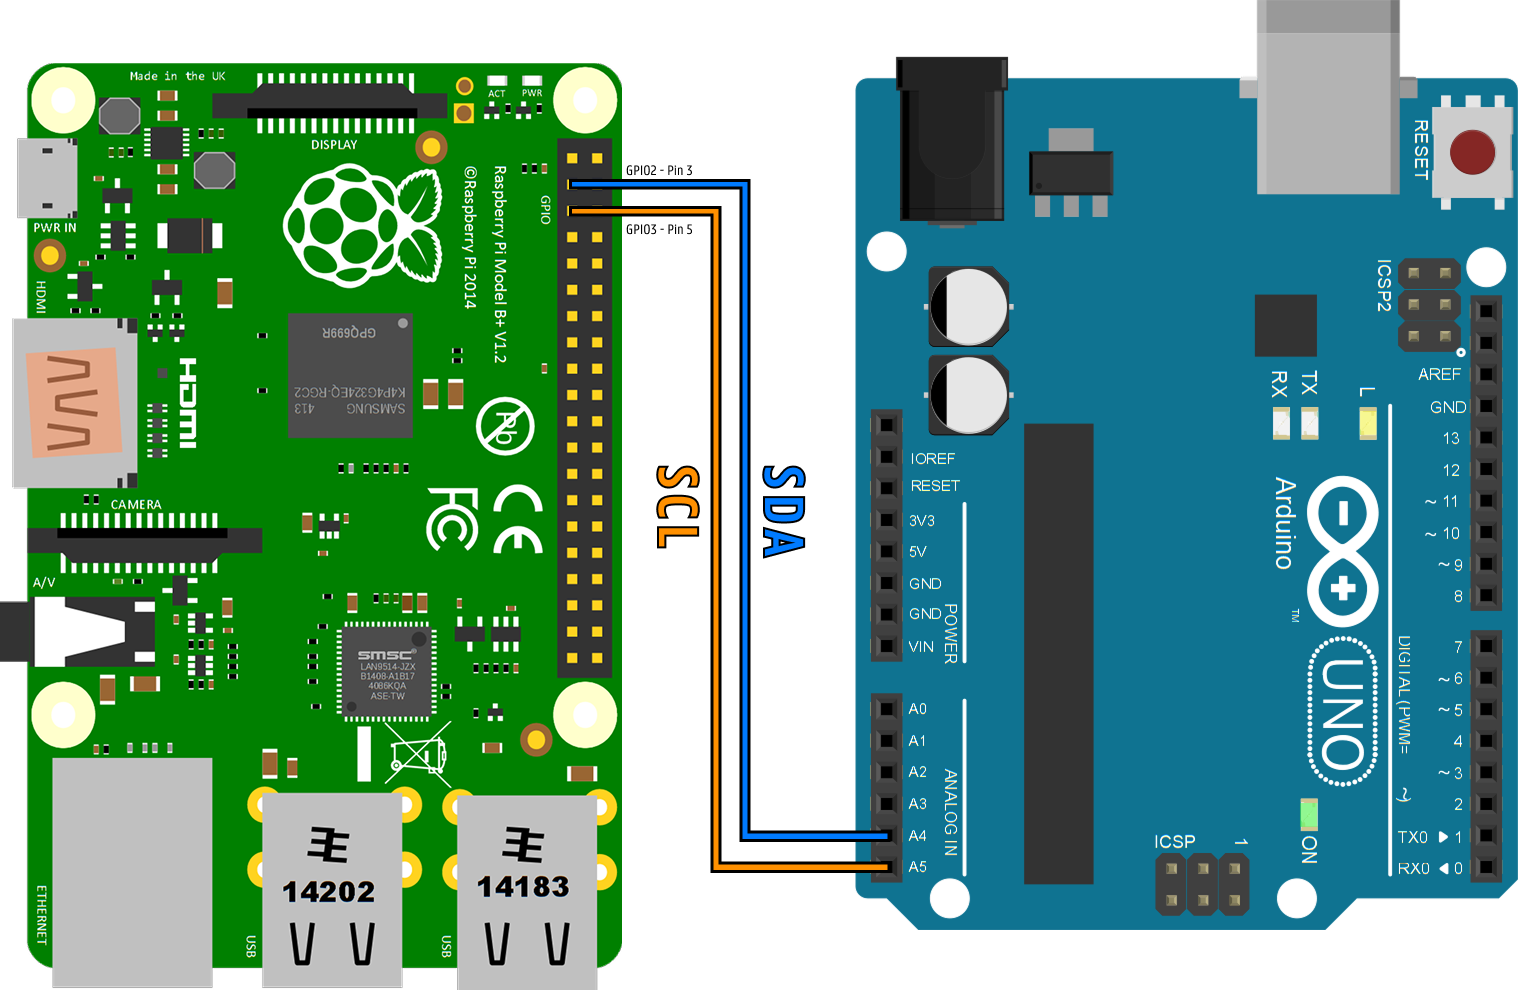
\includegraphics[width=0.7\textwidth]{images/HW_config.png}
	\caption{Hardware connection diagram.}
	\label{fig:hw-connection}
\end{figure}

\subsection{Arduino Firmware Implementation}
\label{subsec:arduino-firmware}

Two firmware versions were developed for different evaluation phases:

\textbf{Correctness Verification Firmware:}
The initial firmware version implements echo functionality with serial output for debugging and correctness verification. This version logs all I2C transactions to the serial monitor, allowing verification of successful read/write operations.

\textbf{Performance Testing Firmware:}
For performance benchmarks, an optimized firmware version was deployed that eliminates serial communication overhead. Upon receiving any I2C write request, the Arduino responds with a fixed ``hello'' message (\texttt{0x68, 0x65, 0x6c, 0x6c, 0x6f}) for one subsequent read operation. This approach minimizes Arduino-side processing variability and keeps extra overhead to a minimum.

\subsection{Benchmark Methodology}
\label{subsec:benchmark-methodology}

The evaluation follows a two-phase methodology to ensure both correctness and measurement reliability.

\subsubsection{Phase 1: Correctness Verification}
\label{subsubsec:correctness-verification}

Prior to performance measurement, functional correctness is verified:
\begin{enumerate}
    \item Deploy correctness verification firmware with serial logging to the Arduino
    \item Execute ping-pong operations across all implementations on the Pi
    \item Verify successful I2C transactions via Arduino Serial Monitor output
\end{enumerate}

\subsubsection{Phase 2: Performance Measurement}
\label{subsubsec:performance-measurement}

Performance evaluation employs \textbf{Criterion.rs}, a statistical benchmarking framework that provides automatic outlier detection, distribution plotting, achievable sample size/mean/deviation/... calculation and more \cite{criterion_rs}. The tool \texttt{cargo-criterion }provides machine-readable JSON output of those measurements, which allows us to also perform manual analysis and visualizations using Python/Jupyter.

We divide the benchmark into three different \textbf{groups}. Each runtime gets evaluated according to the group's implementation:
\begin{itemize}
    \item \textbf{Runtime Setup:} Time to initialize runtime and prepare for I2C operations
    \item \textbf{Cold Execution:} A single ping-pong operation after a new runtime initialization
    \item \textbf{Hot Execution:} Repeated ping-pong operations in steady state
\end{itemize}

\section{Native Implementation - Baseline}
\label{sec:native-baseline}

As the baseline, the native implementation provides reference timing and memory usage characteristics. Visualizing these results is done separately as these axes don't allow cooperation with those from WAMR and Wasmtime results.

\subsection{Native Performance Results}
\label{subsec:native-performance}

Table~\ref{tab:native-performance} presents timing characteristics for the native implementation only using linux-embedded-hal.

\begin{table}[h]
    \centering
    \caption{Native Implementation Performance Characteristics}
    \label{tab:native-performance}
    \begin{tabular}{lrrrr}
        \toprule
        \textbf{Measurement Type} & \textbf{Mean (µs)} & \textbf{Median (µs)} & \textbf{Std Dev (ns)} & \textbf{95\% CI (µs)} \\
        \midrule
        Runtime Setup    & 1.9466 & 1.9483 & 10.5846 & [1.9445 , 1.9487] \\
        Cold Execution   & 594.5275 & 594.5636 & 281.8579 & [594.4715 , 594.5834] \\
        Hot Execution    & 589.0368 & 589.0307 & 69.9196 & [589.0230 , 589.0507] \\
        \bottomrule
    \end{tabular}
\end{table}

% TODO: Add reference naar de appendix met grotere fotos
Figure~\ref{fig:native-distributions} shows the distribution analysis of the Native runtime implementations for each group.
\begin{figure}[h]
    \centering
    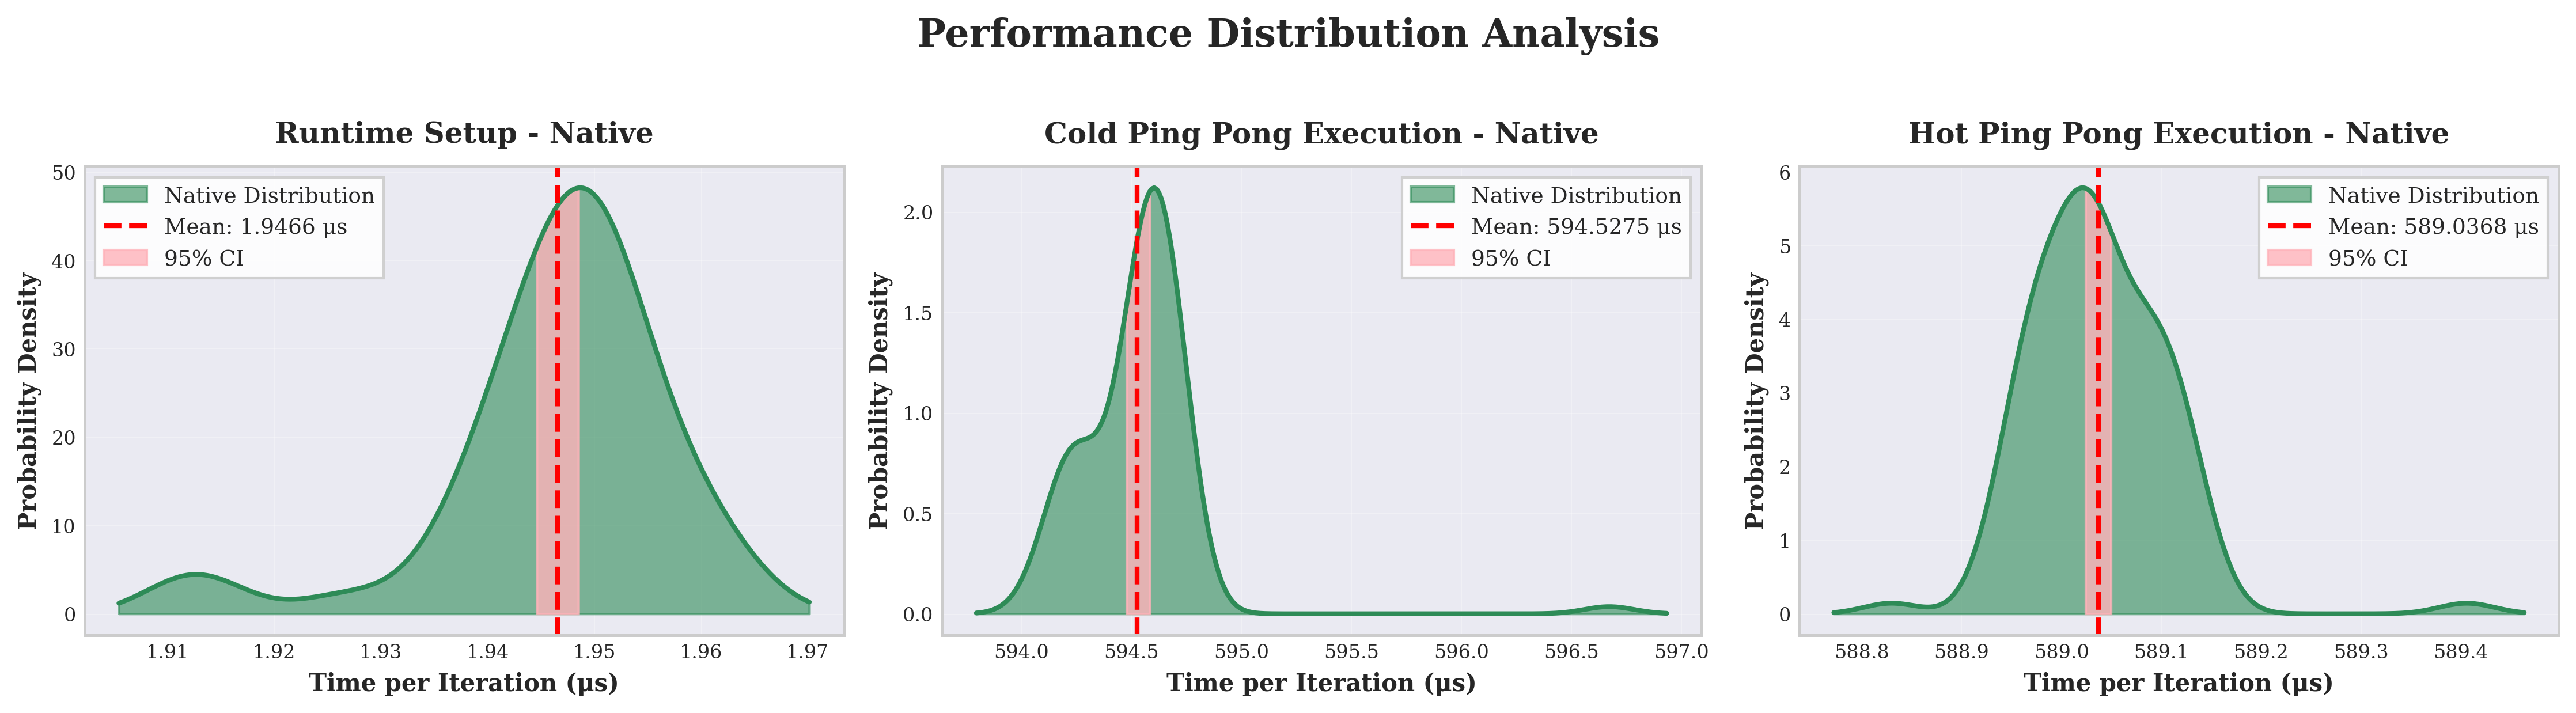
\includegraphics[width=\textwidth]{images/native-distributions}
    \caption{Native Implementation Performance Distribution for each group}
    \label{fig:native-distributions}
\end{figure}

\subsection{Native Memory Usage}
\label{subsec:native-memory}

Table~\ref{tab:native-memory} presents the amount of bytes divided into blocks that were allocated during the setup of the runtime and execution of the routine. Memory profiling reveals minimal allocation overhead for the Native implementation.

\begin{table}[h]
    \centering
    \caption{Native Implementation Memory Characteristics}
    \label{tab:native-memory}
    \begin{tabular}{lrr}
        \toprule
        \textbf{Operation} & \textbf{\#bytes} & \textbf{\#blocks} \\
        \midrule
        Runtime Setup & 10 & 1 \\
        Ping-Pong & 16 & 1 \\
        \bottomrule
    \end{tabular}
\end{table}


\section{WebAssembly Implementations - Performance}
\label{sec:wasm-performance}

The Native implementation is now defined as the baseline. This section presents a detailed performance analysis comparing WAMR and Wasmtime implementations.

\subsection{Runtime Setup}
\label{subsec:wasm-setup-performance}

Table~\ref{tab:wasm-setup-performance} compares runtime initialization overhead between WebAssembly implementations.

\begin{table}[h]
    \centering
    \caption{WebAssembly Runtime Setup Performance}
    \label{tab:wasm-setup-performance}
    \begin{tabular}{lrrrr}
        \toprule
        \textbf{Measurement Type} & \textbf{Mean (µs)} & \textbf{Median (µs)} & \textbf{Std Dev (ns)} & \textbf{95\% CI (µs)} \\
        \midrule
        WAMR          & 253.1126 & 253.1301 & 258.4145 & [253.0613, 253.1638] \\
        Wasmtime      & 19 559.1592 & 19 559.8473 & 11 656.5225 & [19 556.8463, 19 561.4721] \\
        \bottomrule
    \end{tabular}
\end{table}

Figure~\ref{fig:wasm-setup-distributions} shows the distribution analysis of both \acrshort{WASM} Runtime Setups.

\begin{figure}[h]
    \centering
    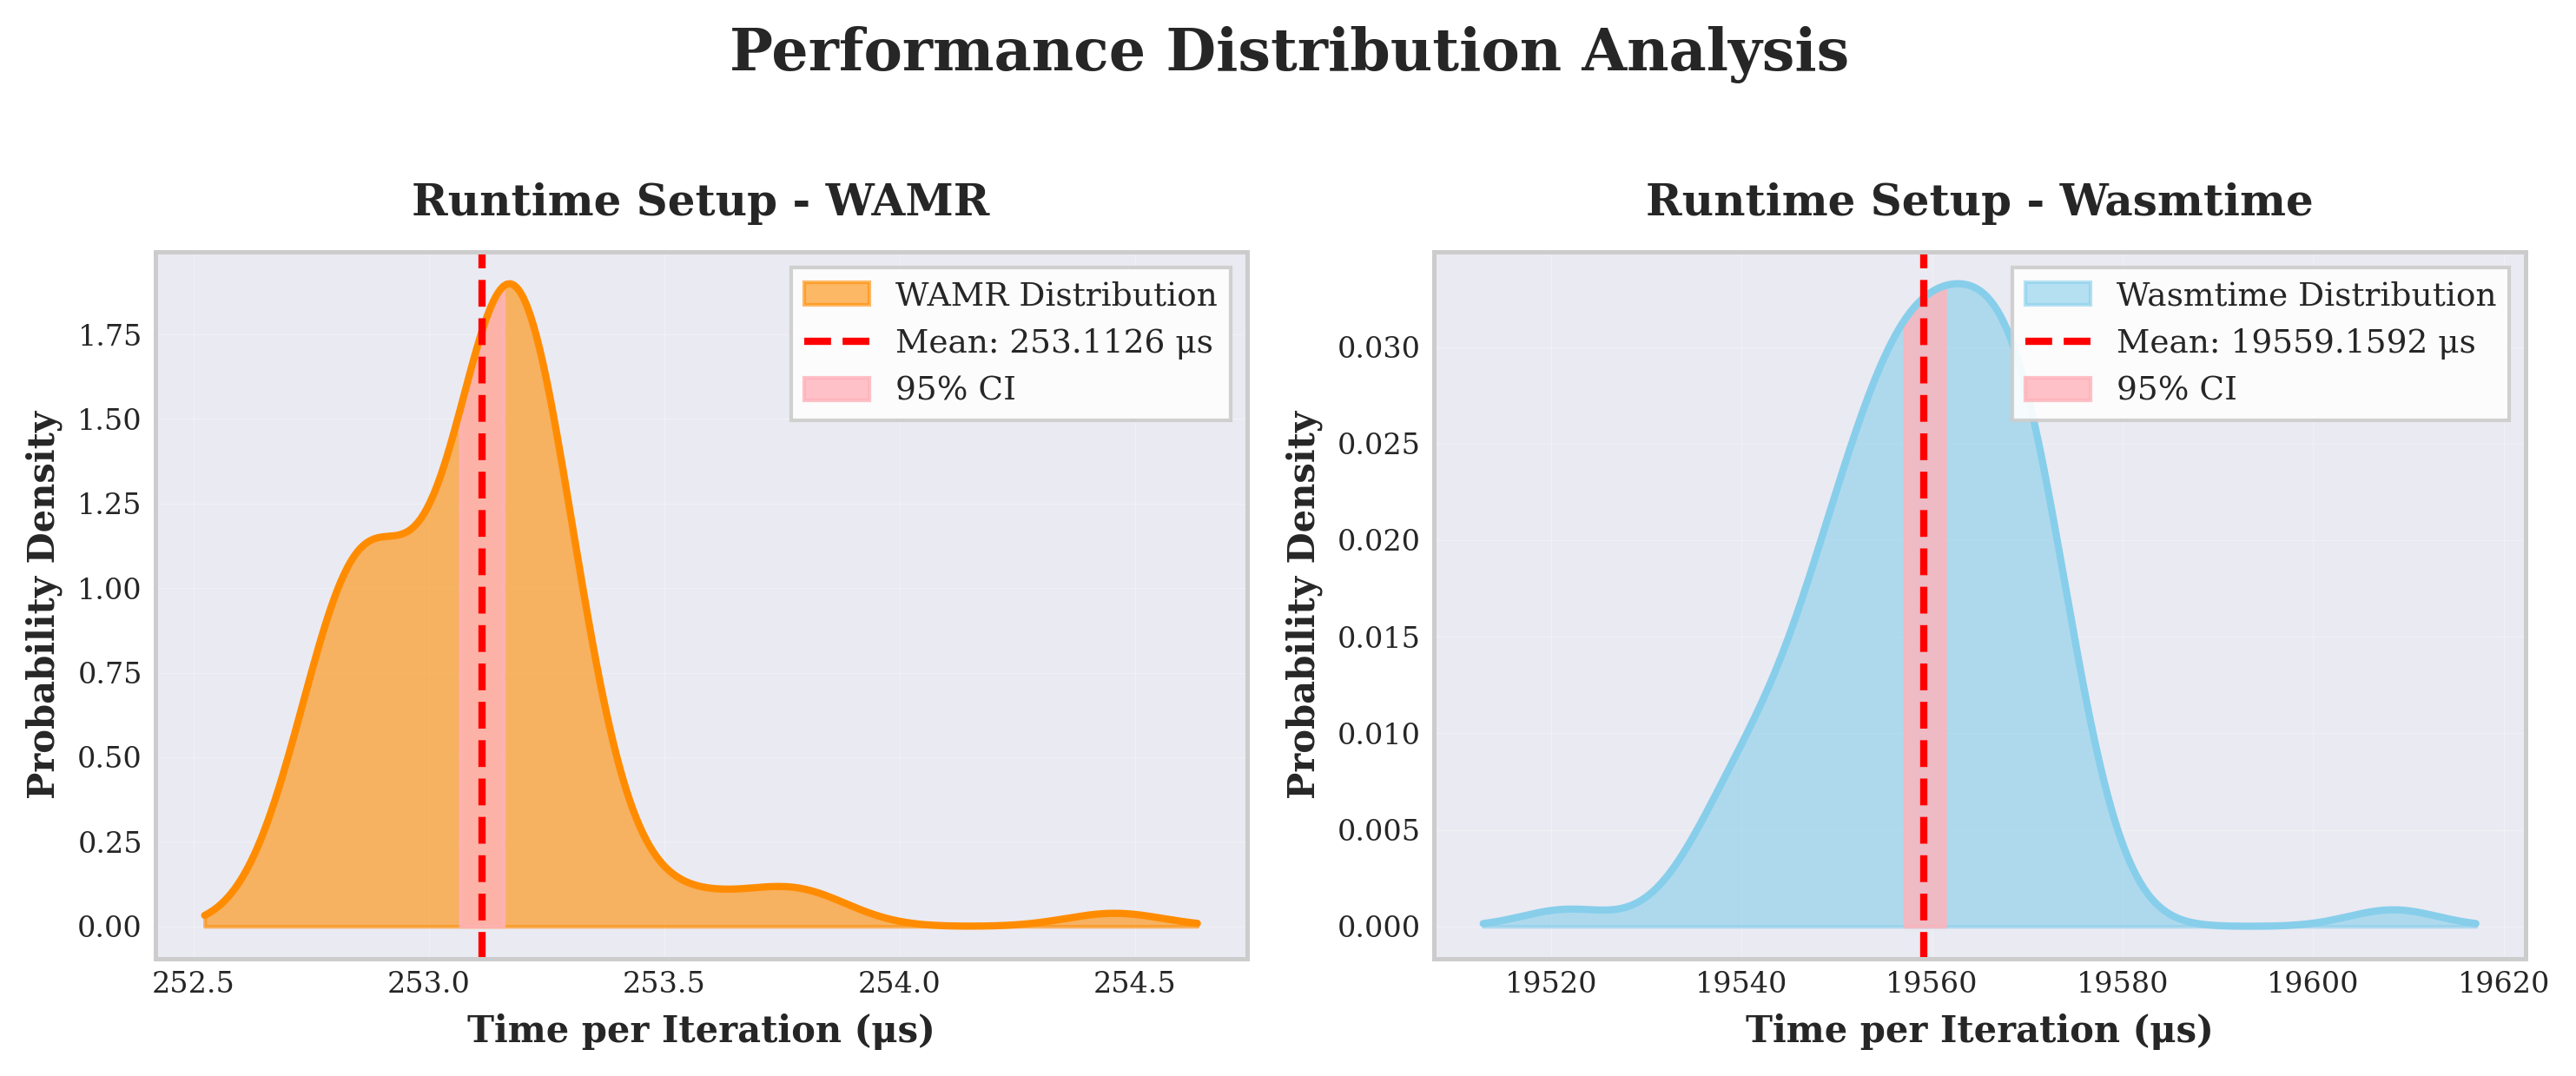
\includegraphics[width=\textwidth]{images/wasm-rt-distributions}
    \caption{\acrshort{WASM} Runtime Setup Performance Distributions}
    \label{fig:wasm-setup-distributions}
\end{figure}



\subsection{Ping Pong Routine}
\label{subsec:wasm-execution-performance}

\subsubsection{Cold Execution}
\label{subsubsec:wasm-cold-execution-performance}

Table~\ref{tab:wasm-cold-execution-performance} presents first-execution performance after runtime initialization.

\begin{table}[h]
    \centering
    \caption{Cold Execution Performance: WAMR vs Wasmtime}
    \label{tab:wasm-cold-execution-performance}
    \begin{tabular}{lrrrr}
        \toprule
        \textbf{Measurement Type} & \textbf{Mean (µs)} & \textbf{Median (µs)} & \textbf{Std Dev (ns)} & \textbf{95\% CI (µs)} \\
        \midrule
        WAMR          & 1 211.0415 & 1 210.9849 & 5 144.4222 & [1 210.0207, 1 212.0622] \\
        Wasmtime      & 1 301.8975 & 1 300.5868 & 4 895.5251 & [1 300.9262, 1 302.8689] \\
        \bottomrule
    \end{tabular}
\end{table}

Figure~\ref{fig:wasm-cold-execution-distributions} shows the distribution analysis of both \acrshort{WASM} Cold Execution routines.

\begin{figure}[h]
    \centering
    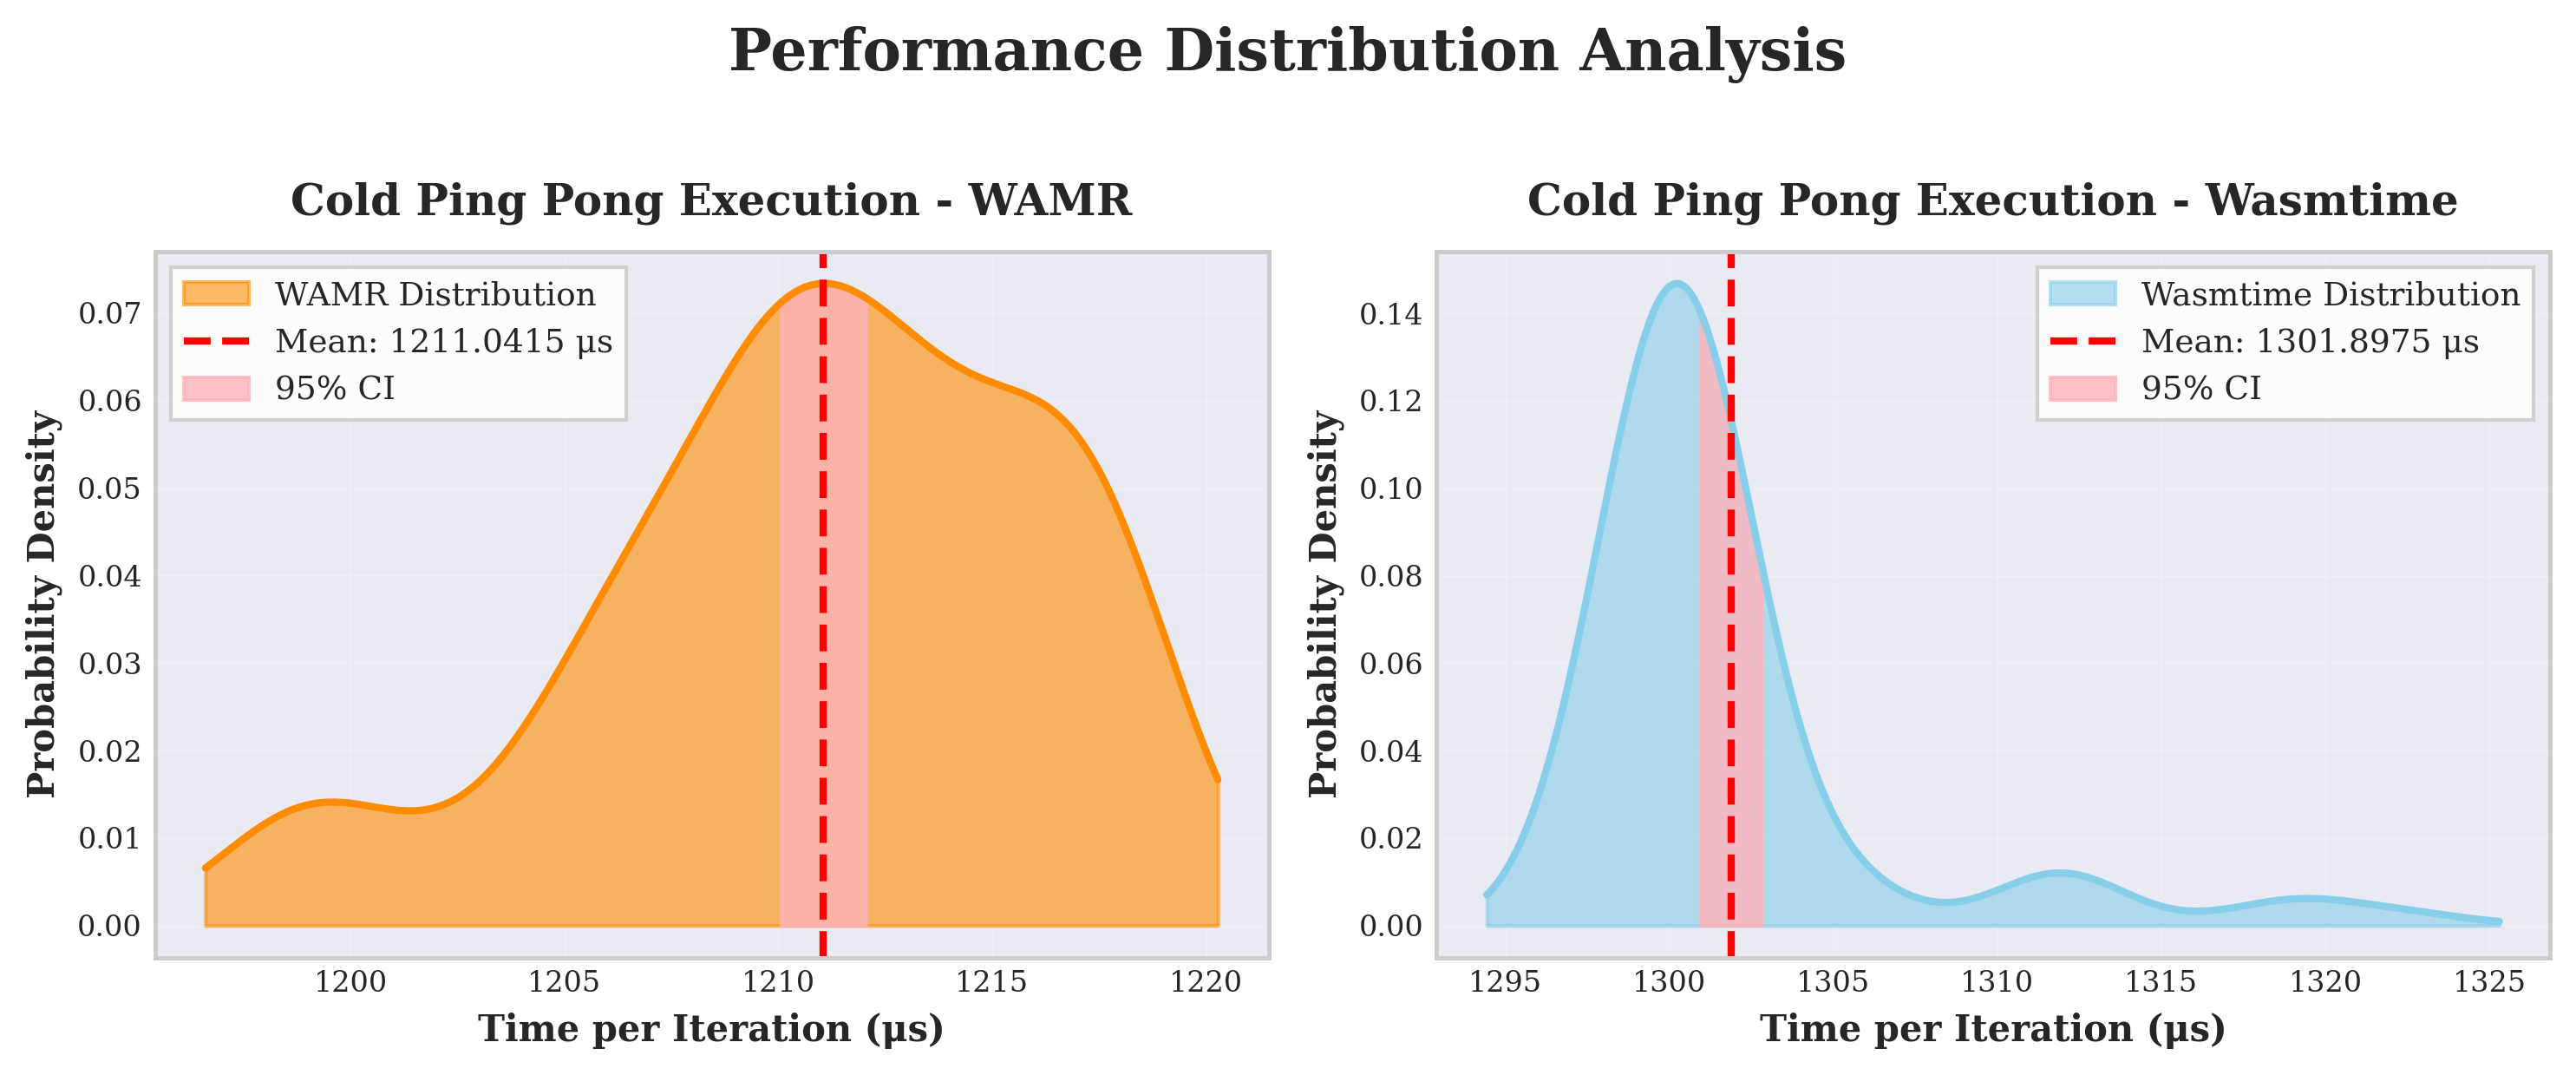
\includegraphics[width=\textwidth]{images/wasm-cold-distributions}
    \caption{\acrshort{WASM} Cold Execution Performance Distributions}
    \label{fig:wasm-cold-execution-distributions}
\end{figure}

\subsubsection{Hot Execution}
\label{subsubsec:wasm-hot-execution}

Table~\ref{tab:wasm-hot-execution-performance} shows steady-state performance characteristics.

\begin{table}[h]
    \centering
    \caption{Hot Execution Performance: WAMR vs Wasmtime}
    \label{tab:wasm-hot-execution-performance}
    \begin{tabular}{lrrrr}
        \toprule
        \textbf{Measurement Type} & \textbf{Mean (µs)} & \textbf{Median (µs)} & \textbf{Std Dev (ns)} & \textbf{95\% CI (µs)} \\
        \midrule
        WAMR          & 1 185.4778 & 1 185.8310 & 673.0608 & [1 185.3442 , 1 185.6113] \\
        Wasmtime      & 1 184.4430 & 1 184.2941 & 522.5048 & [1 184.3393 , 1 184.5467] \\
        \bottomrule
    \end{tabular}
\end{table}

Figure~\ref{fig:wasm-hot-execution-distributions} shows the distribution analysis of both \acrshort{WASM} Hot Execution routines.
\begin{figure}[h]
    \centering
    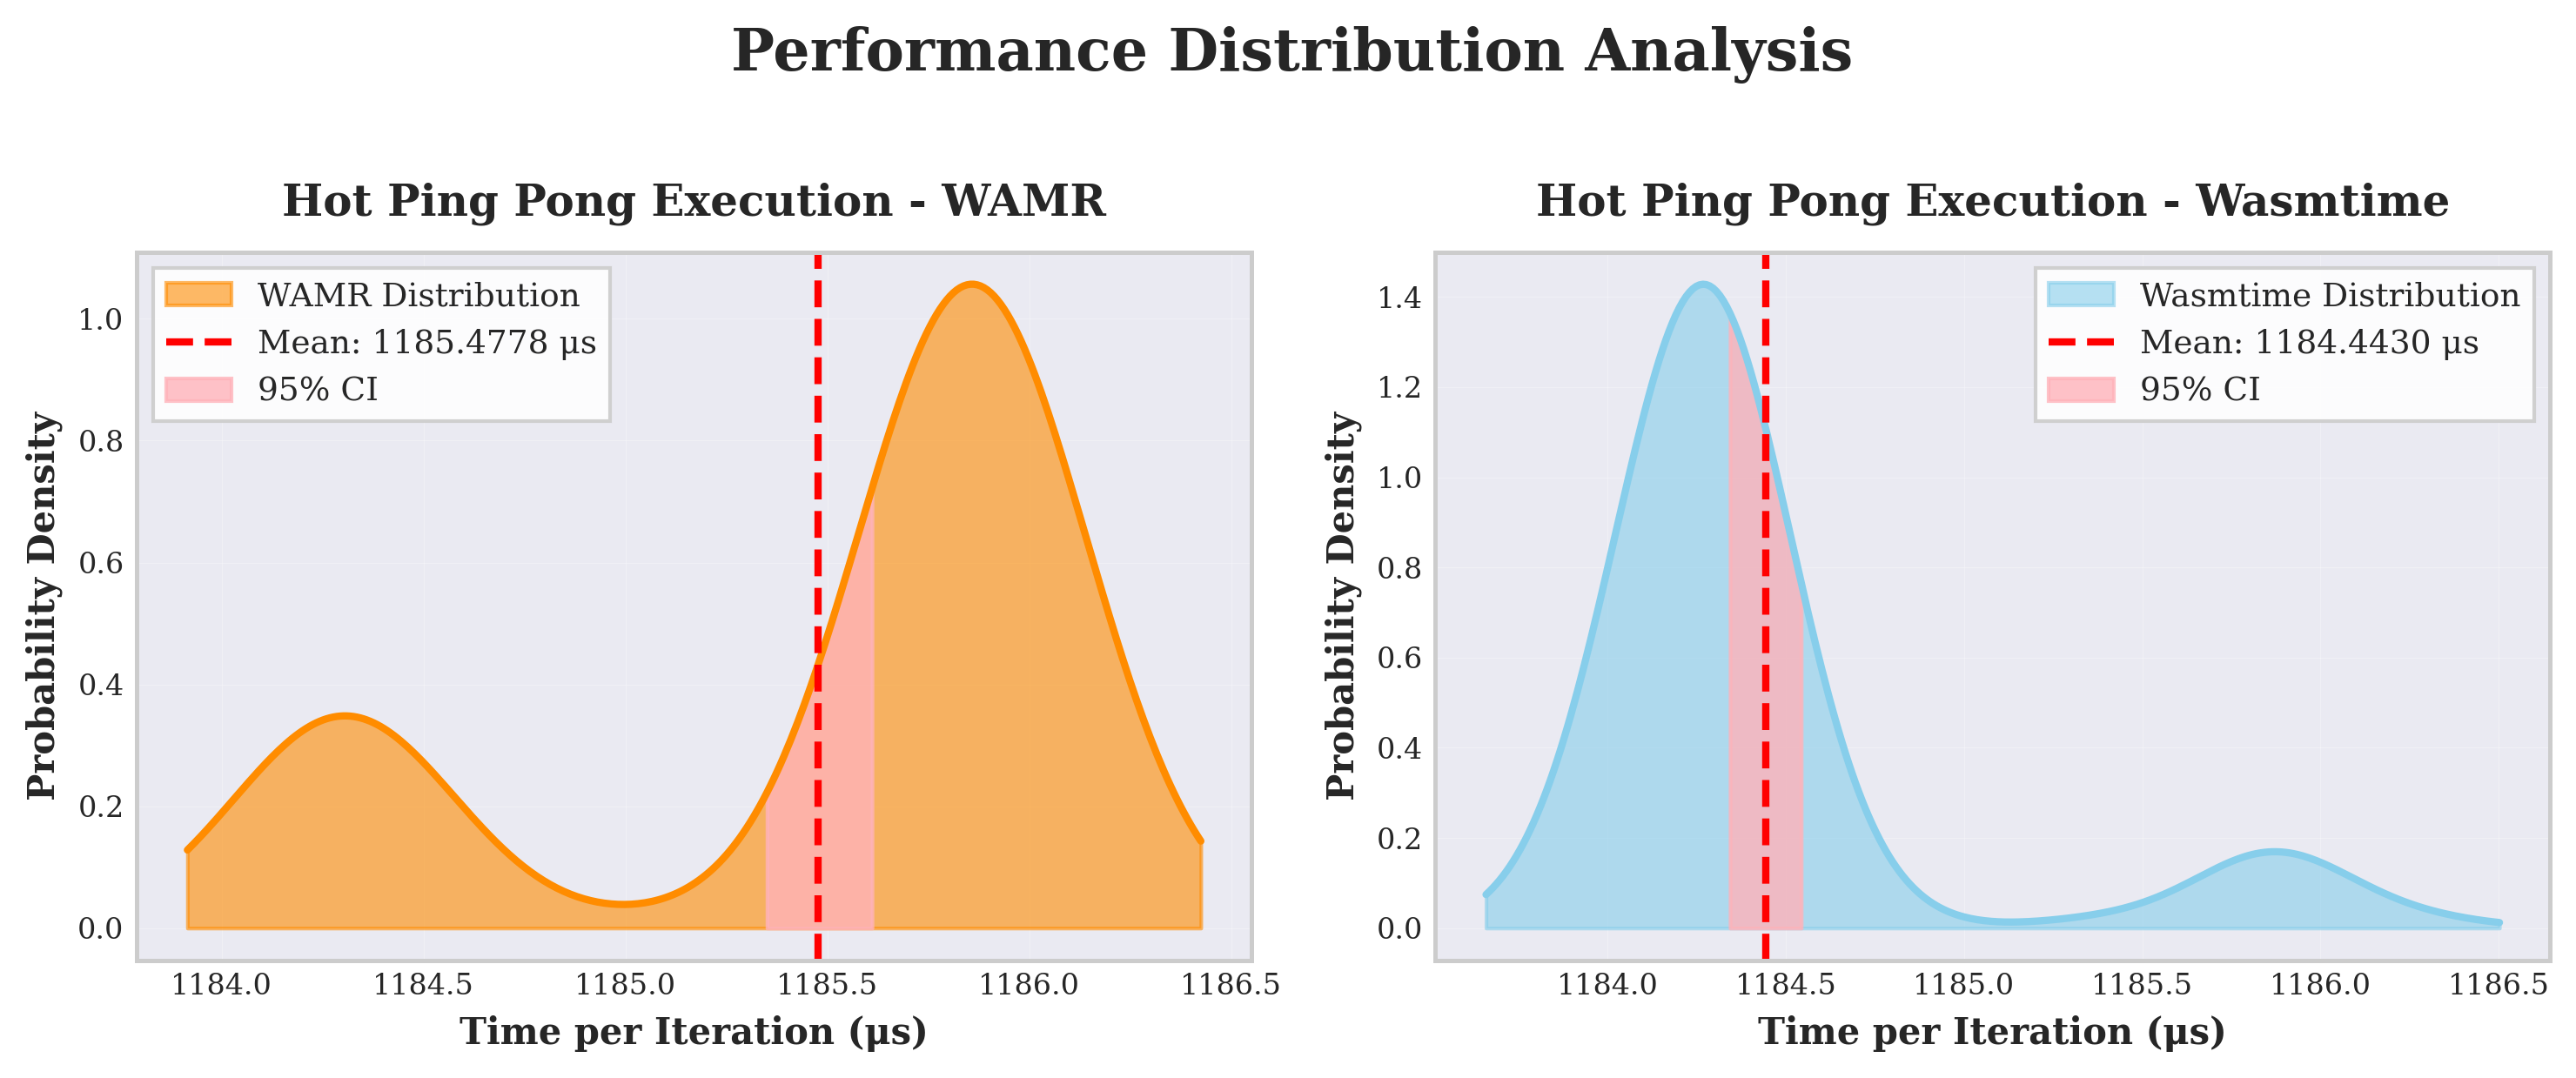
\includegraphics[width=\textwidth]{images/wasm-hot-distributions}
    \caption{\acrshort{WASM} Hot Execution Performance Distributions}
    \label{fig:wasm-hot-execution-distributions}
\end{figure}



% Figure~\ref{fig:wasm-cold-relative} indicates how much slower each Cold Execution routine is compared to the Native baseline.
% \begin{figure}[h]
% \centering
% 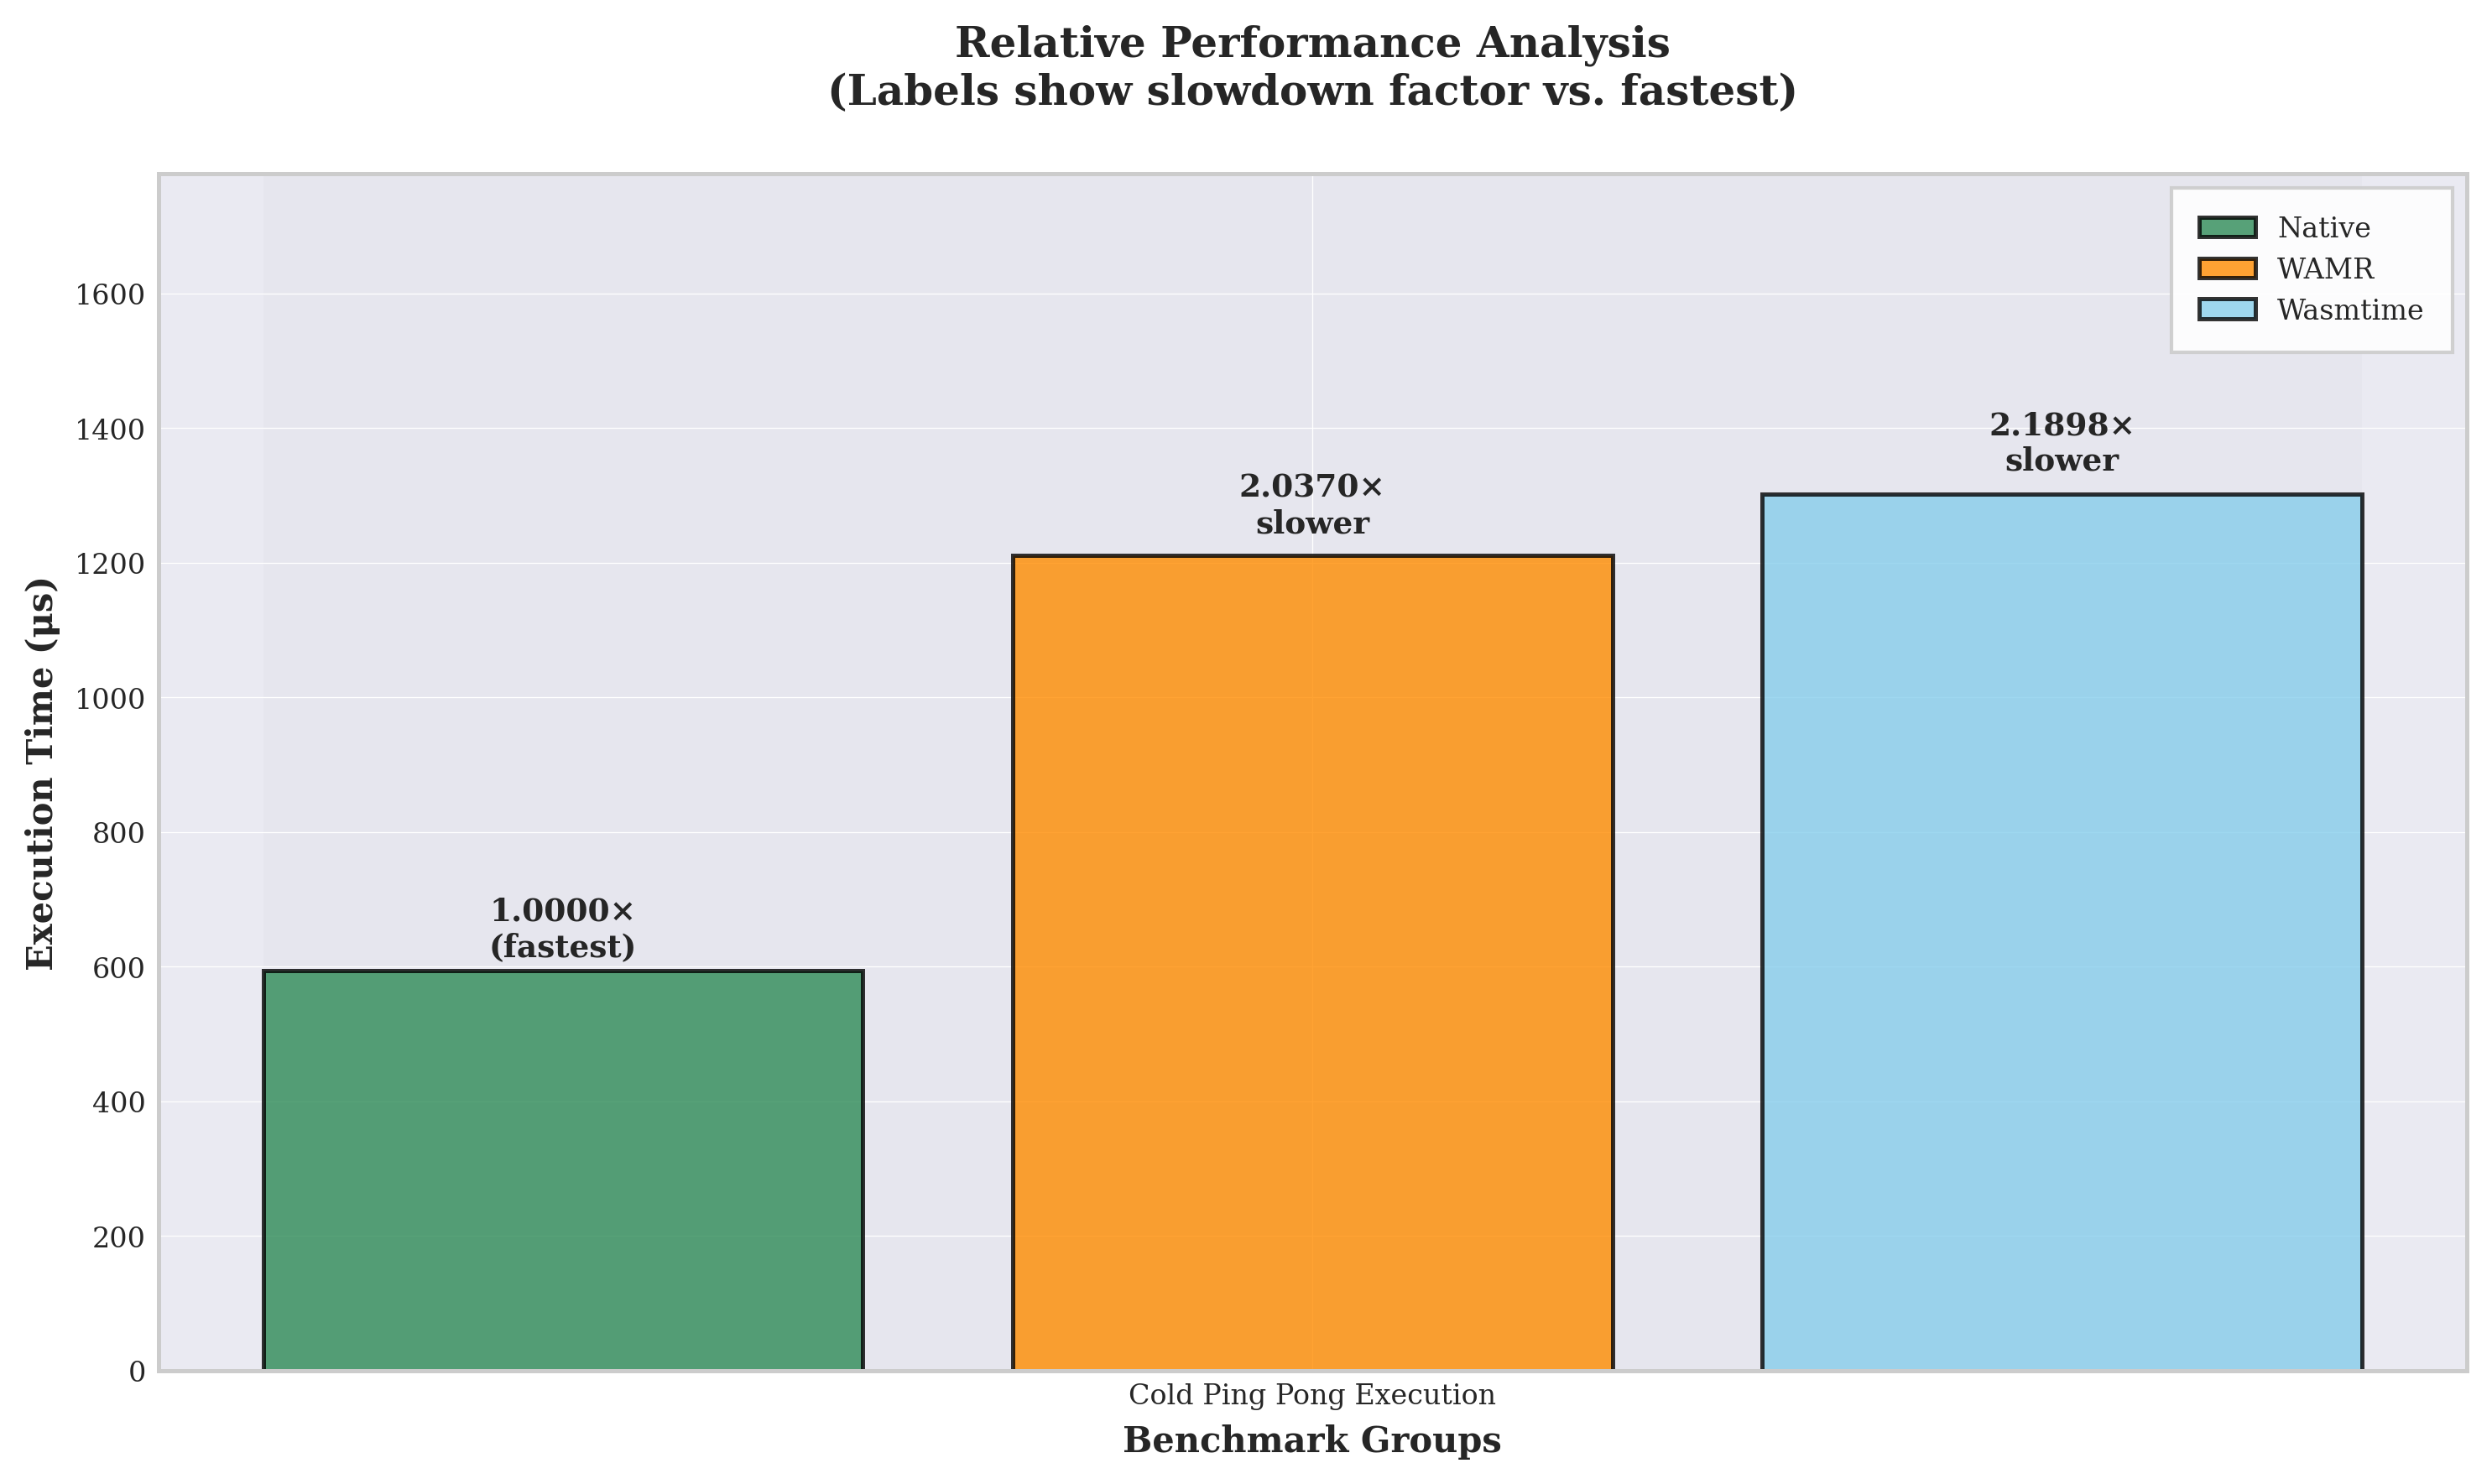
\includegraphics[width=\textwidth]{images/wasm-cold-relative}
% \caption{Relative Performance of Cold Execution routine compared to Native baseline}
% \label{fig:wasm-cold-relative}
% \end{figure}

% Figure~\ref{fig:wasm-hot-relative} indicates how much slower each Hot Execution routine is compared to the Native baseline.
% \begin{figure}[h]
% \centering
% 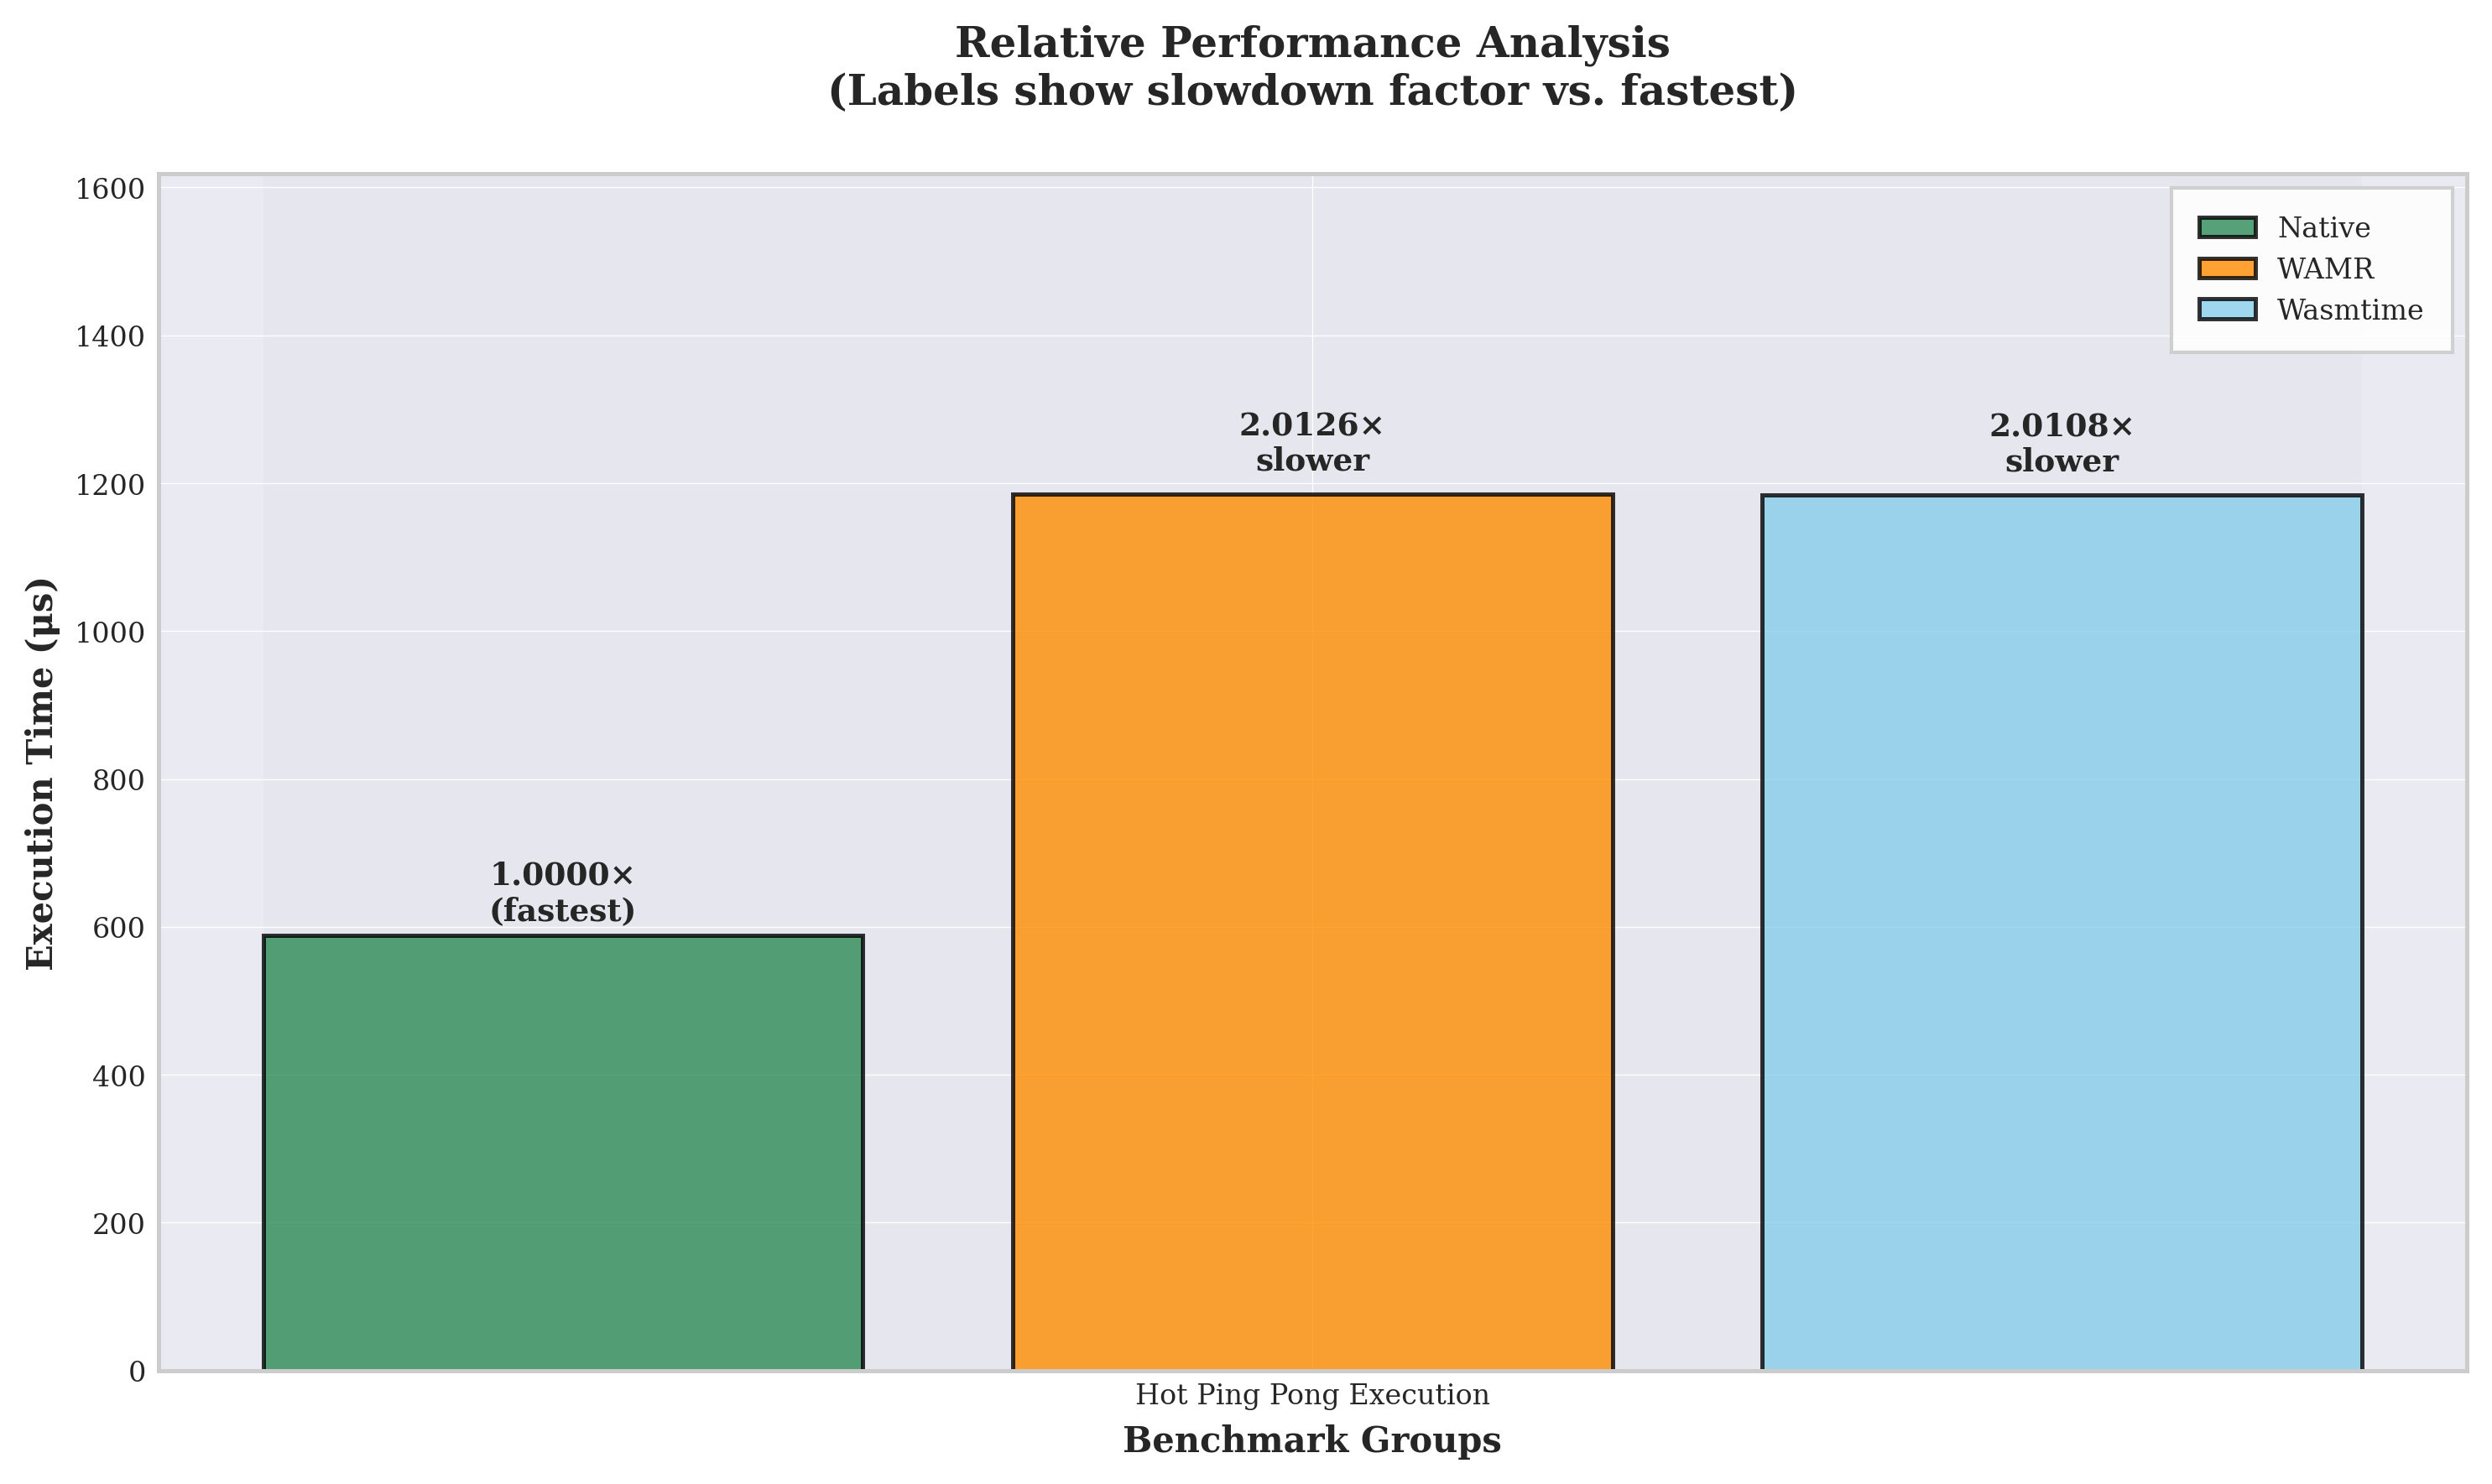
\includegraphics[width=\textwidth]{images/wasm-hot-relative}
% \caption{Relative Performance of Hot Execution routine compared to Native baseline}
% \label{fig:wasm-hot-relative}
% \end{figure}

% Figure~\ref{fig:wasm-rt-relative} indicates how much slower each Runtime Setup is compared to the Native baseline.
% \begin{figure}[h]
% \centering
% 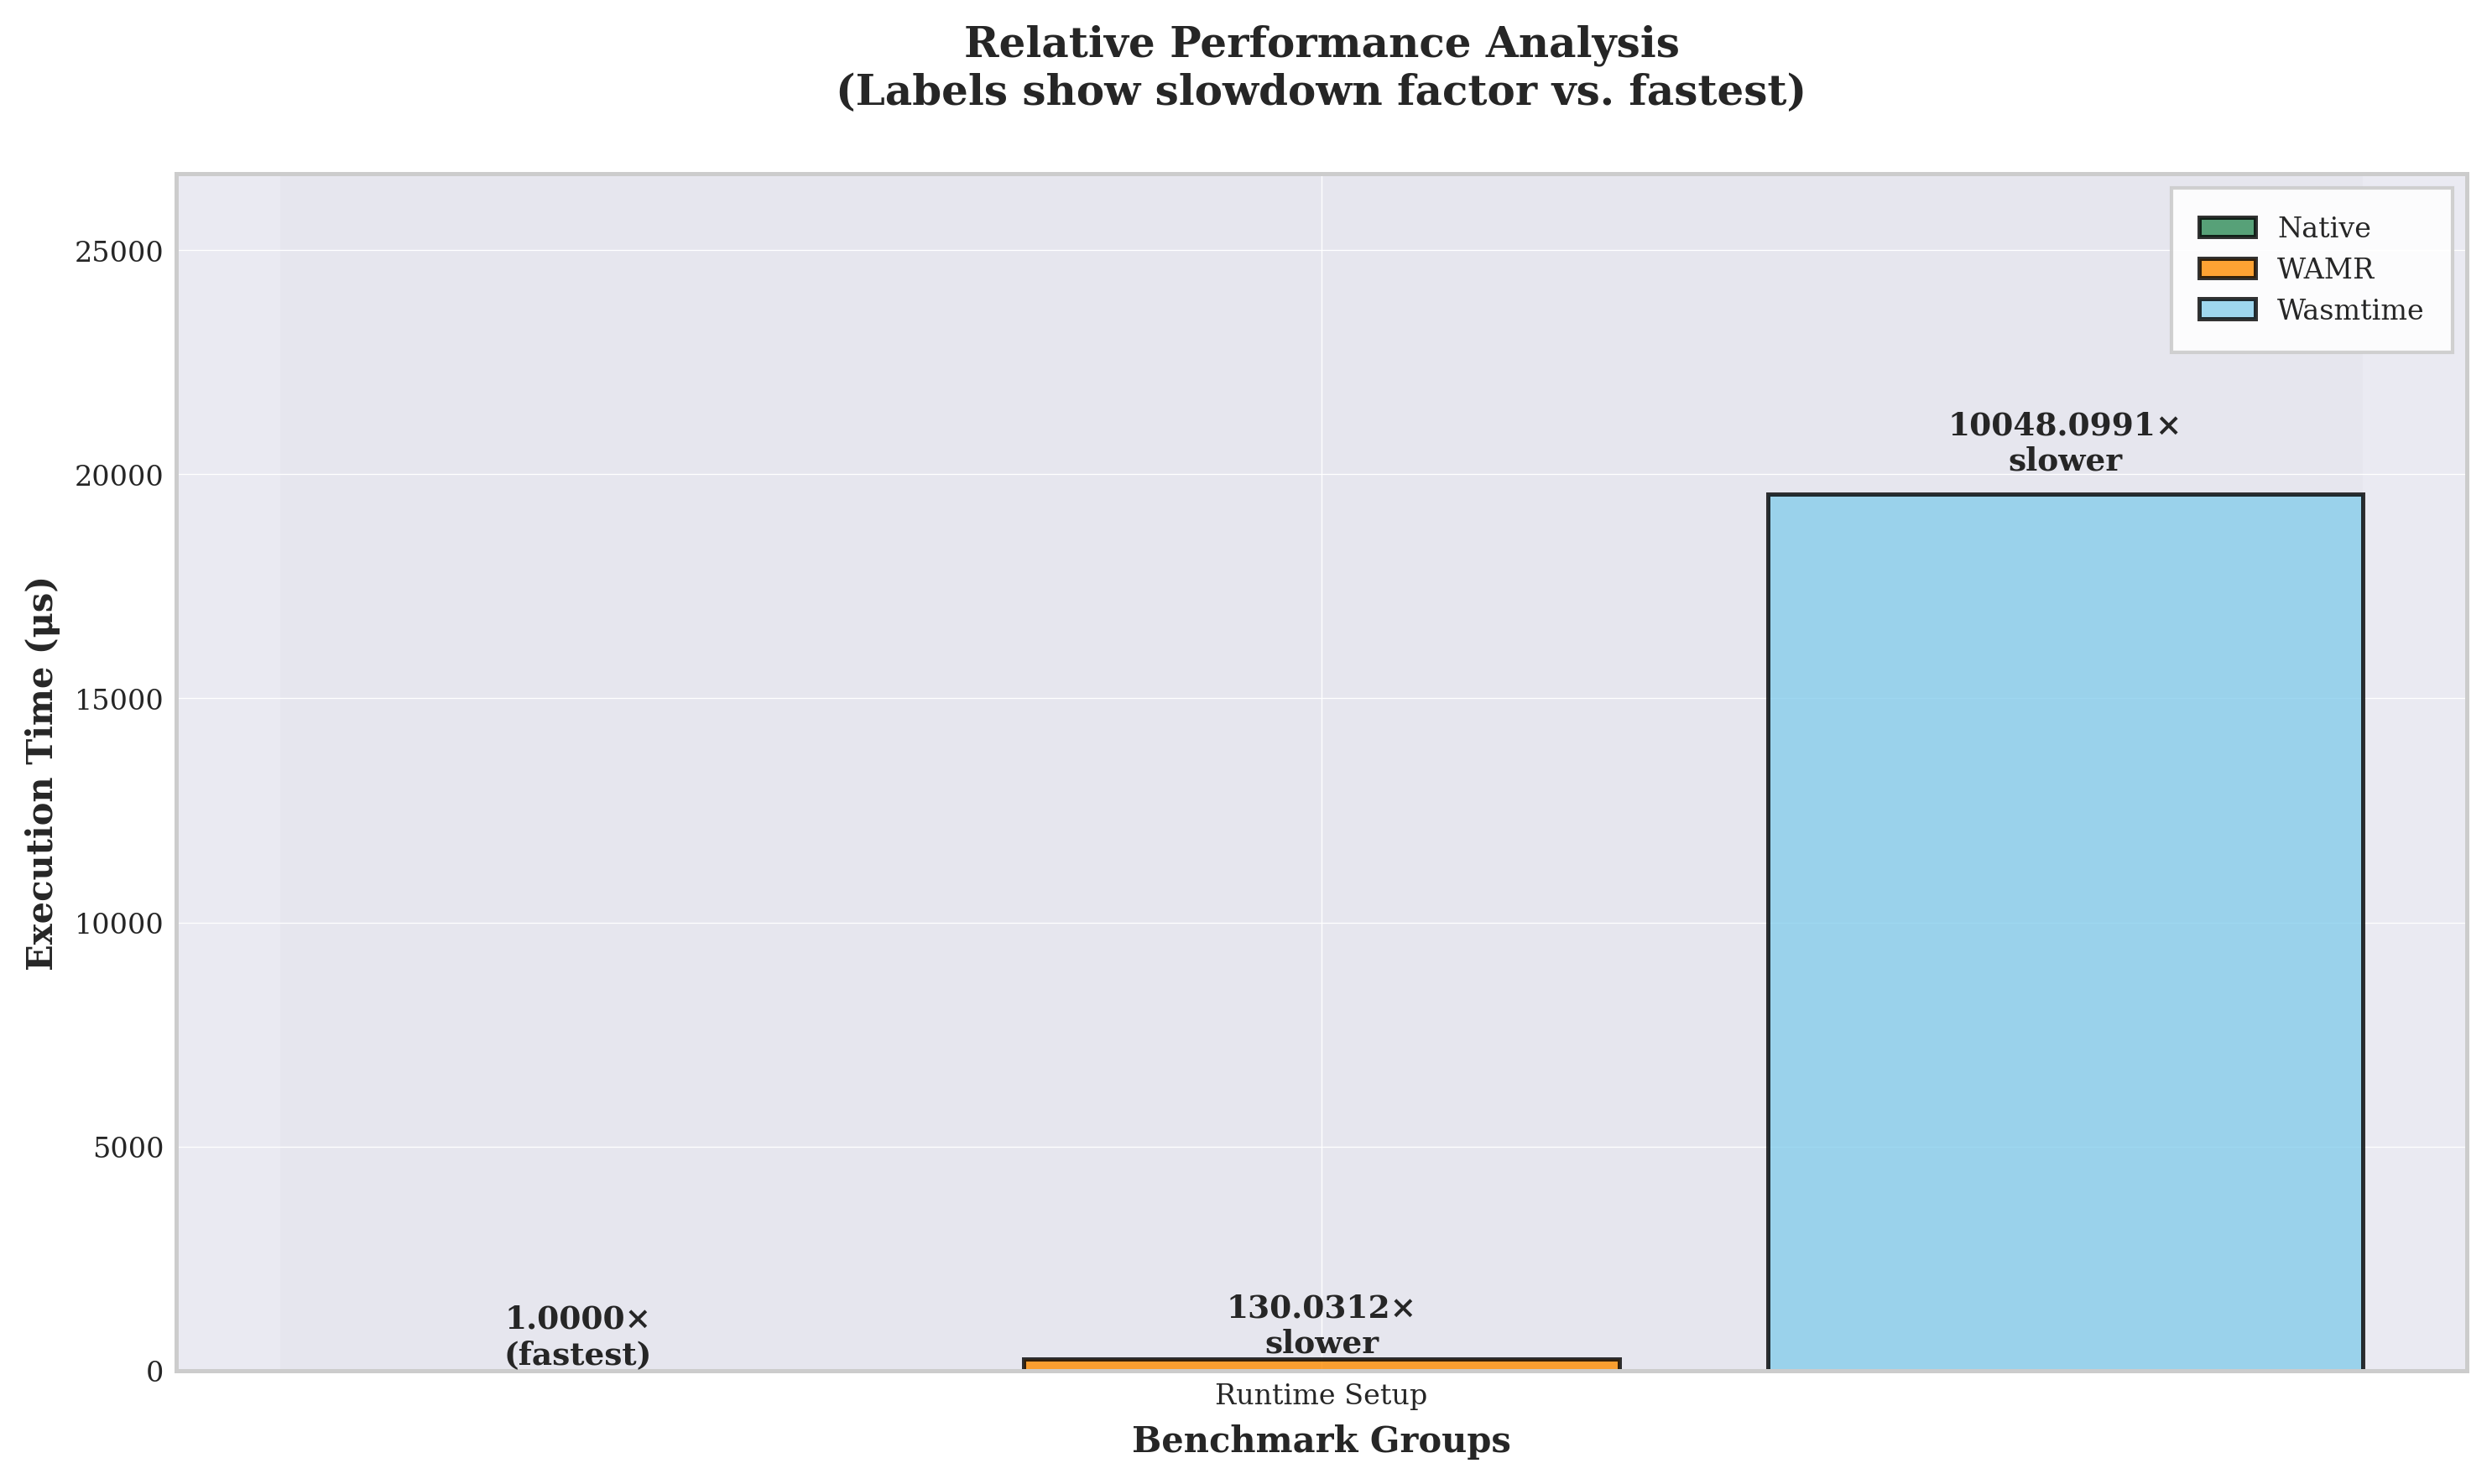
\includegraphics[width=\textwidth]{images/wasm-rt-relative}
% \caption{Relative Performance of Runtime Setups compared to Native baseline}
% \label{fig:wasm-rt-relative}
% \end{figure}











% TODO: Add execution performance comparison figure
% \begin{figure}[htbp]
% \centering
% \includegraphics[width=0.9\textwidth]{figures/execution-performance-comparison}
% \caption{Execution Performance Distribution: WAMR vs Wasmtime}
% \label{fig:execution-comparison}
% \end{figure}

\section{WebAssembly Implementations - Memory}
\label{sec:wasm-memory}

\section{Statistical Analysis}
\label{sec:statistical-analysis}

\subsection{Distribution Characteristics}
\label{subsec:distribution-analysis}

% TODO: Analyze the shape and characteristics of your timing distributions
Performance measurements exhibit distinct distribution characteristics between implementations. 

% TODO: Add distribution comparison figure (box plots/violin plots)
% \begin{figure}[htbp]
% \centering
% \includegraphics[width=1.0\textwidth]{figures/performance-distributions}
% \caption{Performance Distribution Comparison: Box Plots}
% \label{fig:performance-distributions}
% \end{figure}

\textbf{Distribution Analysis:}
% TODO: Describe what the distributions look like
\begin{itemize}
    \item \textbf{WAMR:} \textit{[FILL: describe distribution shape, skewness, outliers]}
    \item \textbf{Wasmtime:} \textit{[FILL: describe distribution shape, skewness, outliers]}
    \item \textbf{Native:} \textit{[FILL: describe distribution shape, baseline variability]}
\end{itemize}

\subsection{Significance Testing}
\label{subsec:significance-testing}

Statistical hypothesis testing evaluates whether observed performance differences are statistically significant.

\textbf{Test Methodology:}
% TODO: Describe your statistical testing approach
\begin{itemize}
    \item \textbf{Test Type:} Mann-Whitney U test (non-parametric, suitable for timing data)
    \item \textbf{Null Hypothesis:} No significant difference between WAMR and Wasmtime performance
    \item \textbf{Significance Level:} $\alpha = 0.05$
    \item \textbf{Effect Size:} Cohen's d for practical significance assessment
\end{itemize}

\textbf{Results:}
% TODO: Report your statistical test results
\begin{itemize}
    \item \textbf{Setup Performance:} $p < \textit{[FILL]}$, $d = \textit{[FILL]}$ (large effect)
    \item \textbf{Cold Execution:} $p = \textit{[FILL]}$, $d = \textit{[FILL]}$ (\textit{[FILL]} effect)
    \item \textbf{Hot Execution:} $p = \textit{[FILL]}$, $d = \textit{[FILL]}$ (\textit{[FILL]} effect)
\end{itemize}

\subsection{Performance Variability Analysis}
\label{subsec:variability-analysis}

Coefficient of variation (CV) quantifies relative variability across implementations:

% TODO: Calculate and report CV values
\begin{equation}
CV = \frac{\sigma}{\mu} \times 100\%
\end{equation}

Table~\ref{tab:variability-analysis} presents variability metrics.

\begin{table}[htbp]
\centering
\caption{Performance Variability Comparison}
\label{tab:variability-analysis}
\begin{tabular}{lrrr}
\toprule
\textbf{Implementation} & \textbf{Setup CV (\%)} & \textbf{Cold Exec CV (\%)} & \textbf{Hot Exec CV (\%)} \\
\midrule
% TODO: Calculate CV for each implementation
Native       & \textit{[FILL]} & \textit{[FILL]} & \textit{[FILL]} \\
WAMR         & \textit{[FILL]} & \textit{[FILL]} & \textit{[FILL]} \\
Wasmtime     & \textit{[FILL]} & \textit{[FILL]} & \textit{[FILL]} \\
\bottomrule
\end{tabular}
\end{table}

\section{Memory Usage Analysis}
\label{sec:memory-analysis}

DHAT profiling provides detailed memory allocation insights across implementation phases.

\subsection{Runtime Setup Memory Profiling}
\label{subsec:memory-setup}

Table~\ref{tab:memory-setup} presents memory allocation characteristics during runtime initialization.

\begin{table}[htbp]
\centering
\caption{Memory Usage During Runtime Setup}
\label{tab:memory-setup}
\begin{tabular}{lrrrr}
\toprule
\textbf{Implementation} & \textbf{Peak Heap (KB)} & \textbf{Total Allocs} & \textbf{Avg Alloc (B)} & \textbf{Max Alloc (B)} \\
\midrule
% TODO: Fill in DHAT setup results
Native        & \textit{[FILL]} & \textit{[FILL]} & \textit{[FILL]} & \textit{[FILL]} \\
WAMR          & \textit{[FILL]} & \textit{[FILL]} & \textit{[FILL]} & \textit{[FILL]} \\
Wasmtime      & \textit{[FILL]} & \textit{[FILL]} & \textit{[FILL]} & \textit{[FILL]} \\
\bottomrule
\end{tabular}
\end{table}

\subsection{Execution Memory Profiling}
\label{subsec:memory-execution}

Table~\ref{tab:memory-execution} shows memory allocation patterns during ping-pong execution.

\begin{table}[htbp]
\centering
\caption{Memory Usage During Ping-Pong Execution}
\label{tab:memory-execution}
\begin{tabular}{lrrrr}
\toprule
\textbf{Implementation} & \textbf{Heap Delta (B)} & \textbf{Exec Allocs} & \textbf{Avg Lifetime (ms)} & \textbf{Fragmentation} \\
\midrule
% TODO: Fill in DHAT execution results
Native        & \textit{[FILL]} & \textit{[FILL]} & \textit{[FILL]} & \textit{[FILL]} \\
WAMR          & \textit{[FILL]} & \textit{[FILL]} & \textit{[FILL]} & \textit{[FILL]} \\
Wasmtime      & \textit{[FILL]} & \textit{[FILL]} & \textit{[FILL]} & \textit{[FILL]} \\
\bottomrule
\end{tabular}
\end{table}

\subsection{Flame Graph Insights}
\label{subsec:flamegraph-analysis}

CPU profiling via flame graph analysis reveals time distribution patterns across function calls.

% TODO: Reference flame graph figure
% \begin{figure}[htbp]
% \centering
% \includegraphics[width=1.0\textwidth]{figures/combined-flamegraph}
% \caption{Combined Flame Graph: CPU Time Distribution}
% \label{fig:flamegraph}
% \end{figure}

% TODO: Brief analysis of flame graph findings
Key observations from flame graph analysis:
\begin{itemize}
    \item \textbf{Hotspot Identification:} \textit{[FILL: major CPU consumers]}
    \item \textbf{Call Stack Depth:} \textit{[FILL: complexity comparison]}
    \item \textbf{I/O vs Computation:} \textit{[FILL: time distribution]}
\end{itemize}

\section{WAMR vs Wasmtime: Detailed Comparison}
\label{sec:detailed-comparison}

This section provides comprehensive analysis of the two WebAssembly runtime approaches.

\subsection{Performance Profile Comparison}
\label{subsec:performance-profiles}

% TODO: Create comprehensive performance comparison
Figure~\ref{fig:performance-radar} presents a multi-dimensional performance comparison.

% TODO: Add radar/spider chart comparing multiple performance aspects
% \begin{figure}[htbp]
% \centering
% \includegraphics[width=0.8\textwidth]{figures/performance-radar-chart}
% \caption{Multi-dimensional Performance Comparison: WAMR vs Wasmtime}
% \label{fig:performance-radar}
% \end{figure}

\textbf{Performance Characteristics Summary:}
\begin{itemize}
    \item \textbf{Startup Latency:} \textit{[FILL: WAMR advantage analysis]}
    \item \textbf{Steady-State Throughput:} \textit{[FILL: execution performance comparison]}
    \item \textbf{Memory Efficiency:} \textit{[FILL: resource usage comparison]}
    \item \textbf{Performance Predictability:} \textit{[FILL: consistency analysis]}
\end{itemize}

\subsection{Architectural Impact Analysis}
\label{subsec:architectural-impact}

\textbf{WASI Preview Differences:}
% TODO: Analyze how Preview 1 vs Preview 2 affects performance
\begin{itemize}
    \item \textbf{Interface Complexity:} \textit{[FILL: binding overhead analysis]}
    \item \textbf{Type System Impact:} \textit{[FILL: WIT vs handwritten binding performance]}
    \item \textbf{Component Model Overhead:} \textit{[FILL: Wasmtime-specific costs]}
\end{itemize}

\textbf{Runtime Architecture Differences:}
% TODO: Discuss implementation differences affecting performance
\begin{itemize}
    \item \textbf{JIT vs Interpretation:} \textit{[FILL: compilation strategy impact]}
    \item \textbf{Memory Management:} \textit{[FILL: allocation strategy differences]}
    \item \textbf{Host Call Mechanisms:} \textit{[FILL: function call overhead]}
\end{itemize}

\subsection{Embedded Systems Suitability}
\label{subsec:embedded-suitability}

\textbf{Resource Constraint Analysis:}
% TODO: Evaluate suitability for embedded applications
\begin{itemize}
    \item \textbf{Memory Footprint:} \textit{[FILL: total memory requirements]}
    \item \textbf{Startup Time Requirements:} \textit{[FILL: real-time application impact]}
    \item \textbf{Deterministic Behavior:} \textit{[FILL: timing predictability]}
    \item \textbf{Power Consumption Implications:} \textit{[FILL: efficiency considerations]}
\end{itemize}

\textbf{Development Experience Comparison:}
\begin{itemize}
    \item \textbf{Toolchain Maturity:} \textit{[FILL: debugging and profiling support]}
    \item \textbf{Standards Compliance:} \textit{[FILL: WASI specification adherence]}
    \item \textbf{Ecosystem Integration:} \textit{[FILL: library and framework support]}
\end{itemize}

\section{Discussion and Implications}
\label{sec:discussion-implications}

\subsection{Key Findings Synthesis}
\label{subsec:key-findings}

% TODO: Synthesize major findings
The experimental evaluation reveals several critical insights:

\begin{enumerate}
    \item \textbf{Setup Performance Divergence:} \textit{[FILL: analysis of extreme Wasmtime setup overhead]}
    \item \textbf{Execution Performance Convergence:} \textit{[FILL: similar steady-state performance]}
    \item \textbf{Memory Usage Trade-offs:} \textit{[FILL: memory vs performance considerations]}
    \item \textbf{Variability Characteristics:} \textit{[FILL: consistency implications]}
\end{enumerate}

\subsection{Practical Application Guidelines}
\label{subsec:application-guidelines}

Based on experimental findings, implementation selection guidelines emerge:

\textbf{Choose WAMR when:}
% TODO: Define WAMR use cases
\begin{itemize}
    \item \textit{[FILL: scenarios where WAMR excels]}
    \item Frequent runtime instantiation required
    \item Memory-constrained embedded environments
    \item Real-time performance requirements
\end{itemize}

\textbf{Choose Wasmtime when:}
% TODO: Define Wasmtime use cases
\begin{itemize}
    \item \textit{[FILL: scenarios where Wasmtime excels]}
    \item Long-running applications (setup cost amortization)
    \item Standards compliance critical
    \item Development velocity prioritized
\end{itemize}

\textbf{Consider Native when:}
% TODO: Define native use cases
\begin{itemize}
    \item Maximum performance required
    \item Platform lock-in acceptable
    \item Security isolation unnecessary
\end{itemize}

\subsection{Performance Optimization Opportunities}
\label{subsec:optimization-opportunities}

% TODO: Identify specific optimization possibilities
Experimental results suggest several optimization directions:

\begin{itemize}
    \item \textbf{Wasmtime Startup Optimization:} \textit{[FILL: potential improvements]}
    \item \textbf{Batch Operation Strategies:} \textit{[FILL: amortizing overhead]}
    \item \textbf{Memory Pool Techniques:} \textit{[FILL: allocation optimization]}
    \item \textbf{Async I/O Integration:} \textit{[FILL: concurrency benefits]}
\end{itemize}

\subsection{Limitations and Validity Threats}
\label{subsec:limitations}

\textbf{Experimental Limitations:}
% TODO: Acknowledge study limitations
\begin{itemize}
    \item \textbf{Workload Scope:} Limited to simple ping-pong I2C operations
    \item \textbf{Hardware Specificity:} Results specific to Raspberry Pi + Arduino setup
    \item \textbf{Scale Considerations:} Single-operation focus may not represent bulk scenarios
    \item \textbf{Environmental Factors:} Controlled laboratory conditions
\end{itemize}

\textbf{Generalizability Considerations:}
\begin{itemize}
    \item \textbf{Architecture Dependence:} ARM64-specific results
    \item \textbf{I2C Protocol Specificity:} May not generalize to other WASI interfaces
    \item \textbf{Implementation Version Sensitivity:} Results tied to specific runtime versions
\end{itemize}

\section{Conclusion}
\label{sec:eval-conclusion}

% TODO: Concise conclusion summarizing key findings
This experimental evaluation provides comprehensive performance characterization of WebAssembly-based I2C implementations. The analysis reveals \textit{[FILL: primary conclusion about WAMR vs Wasmtime trade-offs]} while establishing \textit{[FILL: practical guidelines for implementation selection]}.

Key contributions include:
\begin{itemize}
    \item Quantitative performance comparison across multiple dimensions
    \item Statistical validation of observed performance differences  
    \item Memory usage characterization for embedded applications
    \item Practical guidelines for runtime selection in I2C applications
\end{itemize}

The findings establish a foundation for informed decision-making in embedded WebAssembly I2C applications and identify specific optimization opportunities for future development.

% Professional touches for reproducibility
\section*{Reproducibility Statement}
\label{sec:reproducibility}

All experimental code, benchmark scripts, and raw data are available in the project repository: \texttt{merlijn-sebrechts/wamr-wasi-i2c}. Benchmarks can be reproduced using the provided \texttt{justfile} automation scripts. DHAT profiling and flame graph generation scripts are included in the \texttt{benchall} directory.

% TODO: Add version information table
\begin{table}[htbp]
\centering
\caption{Software Version Information}
\label{tab:software-versions}
\begin{tabular}{lr}
\toprule
\textbf{Component} & \textbf{Version} \\
\midrule
% TODO: Fill in exact versions you used
Rust Toolchain     & \textit{[FILL]} \\
WAMR               & \textit{[FILL]} \\
Wasmtime           & \textit{[FILL]} \\
Criterion.rs       & \textit{[FILL]} \\
DHAT               & \textit{[FILL]} \\
\bottomrule
\end{tabular}
\end{table}